\documentclass[tikz, border=10pt]{standalone}

\usetikzlibrary{arrows}

\begin{document}
	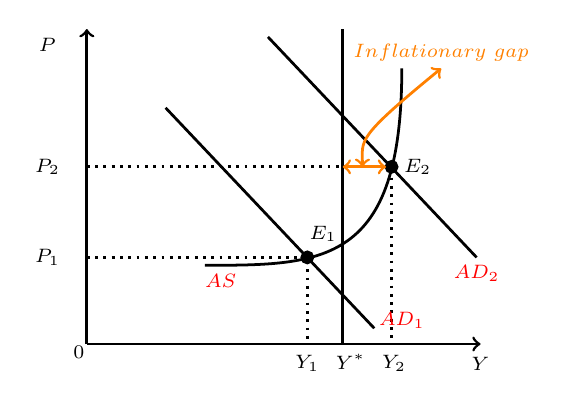
\begin{tikzpicture}[line width=1pt]
	% Нарисовать горизонтальную и вертикальную линии
	\draw[->] (0, 0) -- (5, 0); % Горизонтальная линия
	\draw[->] (0, 0) -- (0, 4); % Вертикальная линия

	\draw (1.5, 1) .. controls (3, 1) and (4, 1) .. (4, 3.5); % Кривая AS
	
	\draw (3.25, 0) -- (3.25, 4); % Линия Y*
	
	\draw[fill=black] (2.8, 1.1) circle (2pt);     % Точки P1-Y1
	\draw[fill=black] (3.87, 2.25) circle (2pt); % Точки P2-Y2
	
	\draw[dotted] (0, 1.1) -- (2.8, 1.1) -- (2.8, 0);          % Линии P1-Y1
	\draw[dotted] (0, 2.25) -- (3.87, 2.25) -- (3.87, 0); % Линии P2-Y2
	
	\draw (1, 3) -- (3.65, 0.2);
	\draw (2.3, 3.9) -- (4.95, 1.1);
	
	\draw[<->, color=orange] (3.25, 2.25) -- (3.8, 2.25);
	\draw[<->, color=orange] (3.5, 2.25) .. controls (3.5, 2.6) and (3.4, 2.6) .. (4.5, 3.5);

	\begin{scriptsize}
		\draw (-0.5, 3.8) node {$P$};
		\draw (5, -0.25) node {$Y$};
		\draw (-0.1, -0.1) node {$0$};
		
		\draw (-0.5, 1.1) node {$P_{1}$};
		\draw (-0.5, 2.25) node {$P_{2}$};
		
		\draw (2.8, -0.25) node {$Y_{1}$};
		\draw (3.35, -0.225) node {$Y^{*}$};
		\draw (3.9, -0.25) node {$Y_{2}$};
		
		\draw[color=red] (1.7, 0.8) node {$AS$};
		\draw[color=red] (4, 0.3) node {$AD_{1}$};
		\draw[color=red] (4.95, 0.9) node {$AD_{2}$};
		
		\draw (3, 1.4) node {$E_{1}$};
		\draw (4.2, 2.25) node {$E_{2}$};
		
		\draw[color=orange] (4.5, 3.7) node {$Inflationary~gap$};
	\end{scriptsize}
	\end{tikzpicture}
\end{document}